\documentclass[11pt,letterpaper]{article}
\usepackage[top=3cm, bottom=2cm, left=2cm, right=2cm, columnsep=20pt]{geometry}
\usepackage{pdfpages}
\usepackage{graphicx}
\usepackage{etoolbox}
\apptocmd{\sloppy}{\hbadness 10000\relax}{}{}
% \usepackage[numbers]{natbib}
\usepackage[T1]{fontenc}
\usepackage{ragged2e}
\usepackage[french]{babel}
\usepackage{listings}
\usepackage{color}
\usepackage{soul}
\usepackage[utf8]{inputenc}
\usepackage[export]{adjustbox}
\usepackage{caption}
\usepackage{amsmath}
\usepackage{amssymb}
\usepackage{float}
\usepackage{csquotes}
\usepackage{fancyhdr}
\usepackage{wallpaper}
\usepackage{siunitx}
\usepackage[indent]{parskip}
\usepackage{textcomp}
\usepackage{gensymb}
\usepackage{multirow}
\usepackage[hidelinks]{hyperref}
\usepackage{abstract}
\usepackage{svg}
\usepackage{biblatex}
\addbibresource{bibliographie.bib}

\renewcommand{\abstractnamefont}{\normalfont\bfseries}
\renewcommand{\abstracttextfont}{\normalfont\itshape}
\usepackage{titlesec}
\titleformat{\section}{\large\bfseries}{\thesection}{1em}{}
\titleformat{\subsection}{\normalsize\bfseries}{\thesubsection}{1em}{}
\titleformat{\subsubsection}{\normalsize\bfseries}{\thesubsubsection}{1em}{}

\usepackage{xcolor}
\definecolor{codegreen}{rgb}{0,0.6,0}
\definecolor{codegray}{rgb}{0.5,0.5,0.5}
\definecolor{codepurple}{rgb}{0.58,0,0.82}
\definecolor{backcolour}{rgb}{0.95,0.95,0.92}
\lstdefinestyle{mystyle}{
    backgroundcolor=\color{backcolour},   
    commentstyle=\color{codegreen},
    keywordstyle=\color{magenta},
    numberstyle=\tiny\color{codegray},
    stringstyle=\color{codepurple},
    basicstyle=\ttfamily\footnotesize,
    breakatwhitespace=false,         
    breaklines=true,                 
    captionpos=b,                    
    keepspaces=true,                 
    numbers=left,                    
    numbersep=5pt,                  
    showspaces=false,                
    showstringspaces=false,
    showtabs=false,                  
    tabsize=2
}
\lstset{style=mystyle}

\usepackage[most]{tcolorbox}
\newtcolorbox{note}[1][]{
  enhanced jigsaw,
  borderline west={2pt}{0pt}{black},
  sharp corners,
  boxrule=0pt, 
  fonttitle={\large\bfseries},
  coltitle={black},
  title={Note:\ },
  attach title to upper,
  #1
}

%----------------------------------------------------

\setlength{\parindent}{0pt}
\DeclareCaptionLabelFormat{mycaptionlabel}{#1 #2}
\captionsetup[figure]{labelsep=colon}
\captionsetup{labelformat=mycaptionlabel}
\captionsetup[figure]{name={Figure }}
\newcommand{\inlinecode}{\normalfont\texttt}
\usepackage{enumitem}
\setlist[itemize]{label=\textbullet}

\begin{document}
\begin{titlepage}
\center

\begin{figure}
    \ThisULCornerWallPaper{.4}{Polytechnique_signature-RGB-gauche_FR.png}
\end{figure}
\vspace*{2 cm}

\textsc{\Large \textbf{PHS3910 --} Techniques expérimentales et instrumentation}\\[0.5cm]
\large{\textbf{Équipe : Lundi 03}}\\[1.5cm]

\rule{\linewidth}{0.5mm} \\[0.5cm]
\Large{\textbf{Écran tactile acoustique}} \\[0.2cm]
\text{Fiche technique du prototype}\\
\rule{\linewidth}{0.2mm} \\[2.3cm]

\large{\textbf{Présenté à}\\
  Jean Provost\\
  Lucien Weiss\\[2.5cm]
  \textbf{Par :}\\
  Émile \textbf{Guertin-Picard} (2208363)\\
  Philippine \textbf{Beaubois} (2211153)\\
  Marie-Lou \textbf{Dessureault} (2211129)\\
  Maxime \textbf{Rouillon} (2213291)\\[3cm]}

\large{\today\\
Département de Génie Physique\\
Polytechnique Montréal\\}

\end{titlepage}

%----------------------------------------------------

\tableofcontents
\pagenumbering{roman}
\newpage

\pagestyle{fancy}
\setlength{\headheight}{14pt}
\renewcommand{\headrulewidth}{0pt}
\fancyfoot[R]{\thepage}

\pagestyle{fancy}
\fancyhf{}
\renewcommand{\headrulewidth}{1pt}
\fancyhead[L]{\textbf{PHS3910}}
\fancyhead[C]{Fiche technique de l'écran tactile acoustique}
\fancyhead[R]{\today}
\fancyfoot[R]{\thepage}

\pagenumbering{arabic}
\setcounter{page}{1}

%----------------------------------------------------

\section{Description générale et spécifications}

Cette fiche technique présente les caractéristiques d'un piano construit avec un
écran tactile acoustique. Un capteur piézoélectrique, sur une plaque de plexiglas 
de 5 mm d'épaisseur, localise un impact par son onde sonore, pour permettre 
de jouer la note appropriée en temps réel. Cette plaque 
et ses dimensions sont présentées à la figure \ref{piano_fig}. Le piano peut jouer\
une seule gamme (12 notes), et est limité à ne pouvoir jouer qu'une seule note à 
la fois. L'acquisition de signal sonore se fait à une fréquence de 44100 Hz par un
ADC, donnant des échantillons de 32 bits. Des fréquences sonores de 0 Hz à 22000 Hz sont présentes. Le délai entre la frappe
et le son de la note est d'environ 200 ms,
dépendant de la puissance de l'ordinateur qui lit les données du capteur. 
 \begin{figure}[H]
   \centering
   
\includegraphics[scale=0.25]{schema.png}
   \caption{Schéma avec dimensions du prototype de piano tactile. Le capteur
   piézoélectrique a son centre positionné à 176 mm du côté gauche et à 207 mm
   du bas de la plaque approximativement.}
   \label{piano_fig}
 \end{figure}

Le tableau \ref{specs} résume les résultats pertinents des tests de caractérisations
effectués sur le prototype. La première ligne du tableau illustre la résolution, la grandeur qu'une note doit prendre pour être distincte, et le 
contraste, qui quantifie la différence entre les signaux obtenus, pour le piano présenté ci-dessus. De là, des bornes ont été posées sur le nombre de bits, la fréquence d'échantillonnage et le contenu fréquentiel
pour évaluer l'influence de chacun sur la performance globale du dispositif. Ces tests ont été effectués dans l'optique d'amoindrir
les coûts pour un deuxième prototype. Les tests choisis dans le tableau \ref{specs} sont ceux pour lesquels la dégradation 
des facteurs résultait en valeurs convenables de résolution et de contraste.

\begin{table}[H]
    \centering
    \begin{tabular}{c c c | c c}
    \hline
    \multicolumn{3}{c|}{Facteurs} & \multirow{2}{*}{Résolution (cm)} & \multirow{2}{*}{Contraste} \\ 
    Bits & Fréq. d'échantillonnage (Hz) & Contenu fréquentiel (Hz) & & \\
    \hline
    32 & 44100 & - & $6.39\ \pm \ 0.08$ & $0.62 \ \pm\ 0.02$ \\
    16 & 44100 & - & $5.0\ \pm \ 0.2$ & $0.70 \ \pm\ 0.08$ \\
    8 & 44100 & - & $4.2 \ \pm\ 0.2$ & $0.58  \ \pm\ 0.09$ \\
    32 & 44100 & 300-5000 & $6.71\ \pm\ 0.08$ & $0.529\ \pm\ 0.004$ \\
    32 & 44100 & 300-1500 &	$6.27\ \pm\ 0.08$ &	$0.72\ \pm\ 0.01$ \\
    32 & 1002 & 10-400 & $5.94\ \pm\ 0.08$ & $0.724\ \pm\ 0.007$  \\
    \hline
    \end{tabular}
    \caption{Tableau des spécifications de l'écran tactile acoustique avec modification de facteurs.\label{specs}}
  \end{table}


\section{Rapports de tests}

La section qui suit détaille les tests effectués afin de produire le tableau des spécifications.
Une attention particulière est portée à la modifications du nombre de bits des échantillons, de
la fréquence d'échantillonage utilisée ainsi qu'au contenu fréquentiel sauvegardé, afin d'analyser
si un dispositif ayant ces facteurs de dégradés peut tout de même présenter des performances adéquates.
Comme c'est le cas, le processeur et la mémoire requise pour opérer le piano pourrait être moins dispendieux
et rester opérationnel.

Les tests mesurent tous la performance du dispositif en analysant la résolution et le contraste, tous les deux
acquis par le processus suivant. Un dictionnaire de plusieurs impacts espacés de 5mm chacuns sur une ligne droite
est enregistrée par le capteur piézoélectrique. Le signal de ces impacts est enregistré sous la forme d'un vecteur.
Un de ces impacts est choisi, puis la corrélation entre ce dernier et tous les impacts est calculée. Afin d'accélérer
le temps de calcul, réduisant ainsi le délai impact-note pour jouer le piano en temps réel, la corrélation est
approximée par un produit scalaire des deux signaux normalisés. Une distribution gaussienne peut ensuite être
ajustée sur les résultats des produits scalaires. Cette dernière permet d'obtenir la résolution par sa largeur à 
mi-hauteur. Un paramètre constant est aussi additionné à la gaussienne afin d'ajuster son "plancher" en hauteur.
La différence entre ce plancher et la valeur du produit scalaire la plus haute est ce qui donne le contraste. Enfin,
ce processus de corrélation entre un signal et le reste du dictionnaire est répété pour différents signaux afin
de faire une étude statistique.
Ainsi, pour chaque tests, le dictionnaire est modifié, puis ce processus de calcul est appliqué. Les calculs
d'incertitudes pour la résolution et le contraste sont détaillés à la section \ref{inc}.

\subsection{Nombre de bits des échantillons du signal}

L'un des tests effectués pour la caractérisation du dispositif est la modification du nombre de 
bits pour les échantillons de chaque signal.
C'est ce nombre qui dicte les grandeurs des sauts possibles entre les valeurs du signal acquis. 
En effet, lorsque le nombre de bits est réduit, la notation en nombres flottants contient moins de décimales,
ce qui fait que moins de nombres réels sont utilisables pour l'approximation de l'amplitude du signal sonore. 
Dans les faits, un bit est toujours réservé pour la description du signe (positif ou négatif).
Puisque la base 2 est utilisée dans ce prototype, le nombre de niveaux disponibles pour approximer
les données est $2^{n -1}$, où $n$ est le nombre de bits alloué au stockage du nombre.
Ainsi, pour diminuer la précision des valeurs du signal au nombre de bits souhaité,
le signal sera multiplié par le facteur $F$ suivant : 
\begin{align}
F=\frac{ 2^{n -1}}{2}\text{.} 
\end{align}
Pour normaliser le signal, chaque
valeur sera ensuite arrondie à son niveau le plus proche. Le signal sera alors divisé par
$F$ 
pour revenir à son échelle d'origine. Avec cette méthode, plusieurs réductions du nombre de bits ont été effectués
sur le dictionnaire original à 32 bits, afin d'essayer de voir si les résultats restent concluants malgré cette
déterioration. Les résultats suivants ont été obtenus et sont présentés dans le tableau \ref{nb_bit_tab}.
\begin{table}[H]
    \centering
    \begin{tabular}{l c c}
    \hline
    Dictionnaire & Résolution (cm) & Contraste  \\ \hline
    1 bits & $0 \pm 8$ & $0 \pm 100$ \\
    2 bits & $0.0 \pm 0.2$ & $0 \pm 5$ \\
    3 bits & $0.04 \pm 0.06$ & $0 \pm 2$ \\
    4 bits & $0.04 \pm 0.03$ & $0 \pm 1$ \\
    6 bits & $0.042 \pm 0.006$ & $0.6 \pm 0.3$ \\
    8 bits & $0.042 \pm 0.002$ & $0.58 \pm 0.09$ \\
    16 bits & $0.050 \pm 0.002$ & $0.70 \pm 0.08$ \\
    32 bits & $0.064 \pm 0.001$ & $0.62 \pm 0.02$ \\
    \hline
    \end{tabular}
    \caption{Tableau de résolution et de contraste en fonction du nombre de bits conservé pour les échantillons.}
    \label{nb_bit_tab}
  \end{table}
  
En analysant les données présentes dans ce tableau, on constate qu'en dessous de 6 bits,  
les valeurs de résolution et de contraste commencent à être nettement moins correctes.  
Cette affirmation peut être démontrée par la nette augmentation des incertitudes, ce qui  
rend les valeurs plus incertaines. De plus, les valeurs de contraste chutent à 0, montrant que les
notes ne sont pas distinctes entre elles. Il est donc juste de déterminer qu'un signal traité  
avec moins de ressources que celles requises pour 6 bits aurait un impact néfaste sur  
l'efficacité du fonctionnement du piano. Cependant, cela nous permet également de remarquer  
qu'un prototype pourrait fonctionner avec moins de bits que le prototype actuel.  
Cela pourrait être bénéfique, car il permettrait de faire fonctionner correctement un prototype  
utilisant moins de mémoire et donc moins de ressources. Cela pourrait permettre de réaliser un projet 
similaire, mais avec des pièces à moindres coûts. 

\subsection{Fréquence d'échantillonnage du signal}

Pour tester différentes fréquences d'échantillonnage plus faibles que la 
fréquence initiale, il suffit d'échantilloner l'échantillon déjà obtenu. En
effet, en prenant un point sur deux dans un échantillon dont la fréquence
d'échantillonnage est de 44 100 Hz, le nouvel échantillon a directement une
fréquence d'échantillonnage de 22 050 Hz. 
En procédant de cette façon, plusieurs fréquences d'échantillonnage ont été
artificiellement enregistrées. Les résultats de résolution et contraste 
qu'elles ont produits sont présentés au tableau \ref{fs_fig}.

\begin{figure}[H]
    \centering
    \includegraphics[scale=0.55]{graphique_fs.png}
    \caption{Contraste et résolution en fonction de la fréquence d'échantillonnage.}
    \label{fs_fig}
\end{figure}

26 valeurs de fréquences été testées, mais seules les valeurs non aberrantes sont
présentes sur le graphique. La ligne pointillée verticale indique 
la moitié des valeurs testées. On constate  que peu de valeurs sont affichées
pour une fréquence en dessous de 400 Hz. Cela est dû à des aberrations dans
la convergence du fit gaussien utilisé dans le code, ce qui témoigne de 
données d'une qualité insuffisante pour être utilisé dans la conception d'un
piano. 
On remarque également que la fréquence et le contraste varient légèrement entre 
400 Hz et 44,1 kHz, mais qu'il n'y a pas de tendance à la hausse ou à la baisse 
générale. Cela indique qu'on peut diminuer la fréquence d'échantillonnage 
jusqu'à 400 Hz sans trop d'impact sur la résolution et le contraste, permettant
l'utilisation de processeurs nettement moins puissants et coûteux que ceux d'ordinateurs
personnels.

\subsection{Contenu fréquentiel du signal}

Pour stocker le signal, il est possible de le transformer dans le domaine 
fréquentiel, puis d'en retirer une partie avant de l'enregistrer. De cette 
façon, un moins grand nombre de bit est nécessaire pour conserver l'information.

Le processus pour retirer une partie du contenu fréquentiel du signal consiste
à lui appliquer une FFT, puis à définir des filtres à appliquer, d'obtenir le
signal fréquentiel filtré et enfin appliquer la FFT inverse pour retrouver
un signal dans le domaine temporel ayant un contenu fréquentiel réduit. 
Il est alors possible de tester la qualité de ce nouveau signal en calculant
la résolution et le contraste obtenu à l'aide d'une corrélation avec un 
ensemble de vecteurs ayant été réduits de la même façon. 

Le filtre dans le domaine fréquentiel est défini à l'aide de fonctions de 
Heaviside, qui retourne zéro comme valeur jusqu'au paramètre et 1 pour des valeurs 
strictement supérieures au paramètre.
Le filtre passe-haut, qui détermine la fréquence minimale conservée, est directement
une fonction de Heaviside, alors que le filtre passe-bas, qui détermine la fréquence 
maximale conservée, est une fonction de Heaviside inversée en x, c'est-à-dire que ce 
sont les valeurs supérieures ou égales au paramètre du filtre qui sont nulles et les
valeurs strictement inférieures qui sont égales à 1. Le filtre final est la somme des
deux filtres, ce qui forme une fonction fenêtre.
En multipliant terme à terme le filtre et le vecteur dans le domaine fréquentiel, on 
obtient le vecteur filtré dont les composantes sont conservées lorsqu'elles sont dans 
à l'intérieur de l'intervalle et nulles sinon.

En modifiant la valeur des filtres, on peut voir l'impact de la réduction du contenu 
fréquentiel sur la résolution et le contraste afin de déterminer jusqu'à quelles 
fréquences on peut réduire le signal. La fréquence maximale conservée est le premier
paramètre testé et ses résultats sont illustrés à la figure \ref{fmax_fig}, pour une 
fréquence minimale conservée de 10 Hz et une fréquence d'échantillonnage de 44,1 kHz.

\begin{figure}[H]
    \centering
    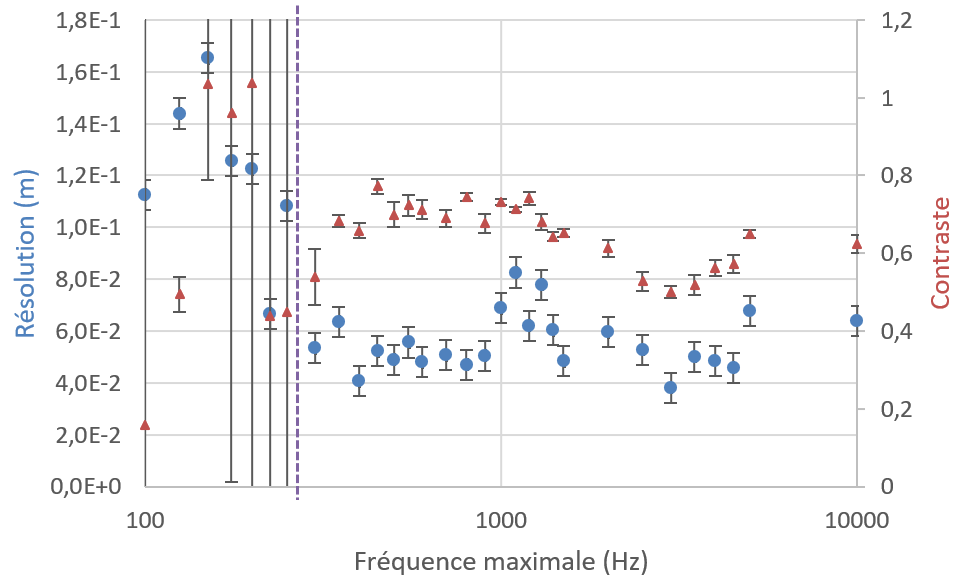
\includegraphics[scale=0.55]{Freqmax_graph.png}
    \caption{Contraste et résolution en fonction de la fréquence maximale conservée.}
    \label{fmax_fig}
\end{figure}

On observe que dans la portion à droite de la ligne pointillée verticale, le 
contraste est relativement constant autour de 0,7 entre $0,50 \pm 0,02$ et $0,80 \pm 0,02$ et 
la résolution est également relativement constante autour de 6cm entre $(8,3 \pm 0,1)$ cm et 
$(4,0 \pm 0,1)$ cm. Dans la portion à gauche de la ligne pointillée, les valeurs 
fluctuent beaucoup plus, avec des résolution qui dépassent 10 cm, des incertitudes 
supérieures aux valeurs et même des contrastes obtenus avec la régression gaussienne
qui dépassent 1. Ces éléments correspondent à un échec de la régression gaussienne 
et témoignent d'une trop grande dégradation du signal. La position de la ligne 
pointillée, à environ 300 Hz, marque une limite inférieure pour la réduction de 
la fréquence maximale conservée.

De la même façon, on peut tester la fréquence minimale conservée en fixant la 
fréquence maximale à 5000 Hz et la fréquence d'échantillonnage à 44,1 kHz. Les 
résultats de ce test sont présentés à la figure \ref{fmin_fig}.

\begin{figure}[H]
    \centering
    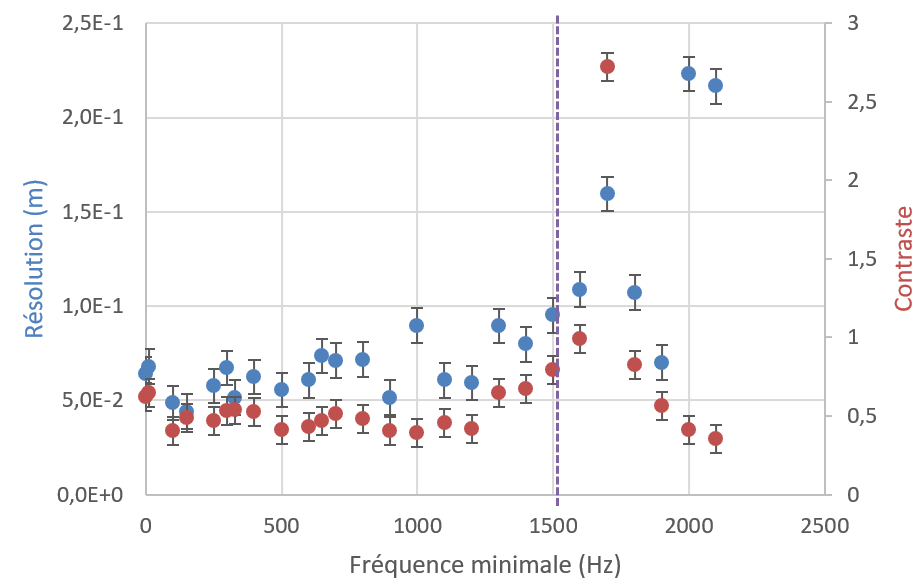
\includegraphics[scale=0.55]{Freqmin_graph.png}
    \caption{Contraste et résolution en fonction de la fréquence minimale conservée.}
    \label{fmin_fig}
\end{figure}

À gauche de la ligne pointillée verticale, on observe des valeurs relativement 
constantes pour la résolution et le contraste, soit respectivement autour de 6 cm,
entre ($4,4 \pm 0,1$) cm et ($9,5 \pm 0,8$) cm et autour de 0,5 entre 
$0,41 \pm 0,1$ et $0,8 \pm 0,4$. À droite de la ligne pointillée, le même 
comportement divergent peut être observé, avec des résolutions et des contrastes 
qui sont plus du doubles des valeurs attendues et des incertitudes très grandes par 
endroit. À nouveau, la position de la ligne pointillée à environ 1500 Hz marque la 
limite supérieure pour l'augmentation de la fréquence minimale conservée.

En considérant ces deux résultats conjointement, il est clair qu'ils ne peuvent pas 
être implémentés simultanément, puisque cela conduirait à un signal totalement nul. 
En se rappelant l'objectif de ces tests, soit de voire à réduire au maximum la 
quantité d'information à enregistrer, une préférence est développée pour les filtres
limitant au maximum la bande de fréquences nécessaire pour obtenir un 
résultat équivalent au piano réalisé au préalable. Comme la limitation imposée à la
fréquence maximale est la plus grande des deux, réduisant à environ 400 Hz le 
spectre de fréquences plutôt qu'à environ 20kHz ($20 550=22 050 - 1500$), c'est la 
configuration de ce test qui est choisie. 
Le contenu fréquentiel peut donc être restreint à l'intervalle [10,400] Hz pour sauver de la
mémoire.

% \begin{table}[ht]
%     \centering
%     \begin{tabular}{c c c}
%     \hline
%     fréquence minimale (Hz) & Résolution (cm) & Contraste  \\ \hline
%     0 & $0.064 \pm 0.001$ & $0.62 \pm 0.02$ \\
%     400 & $0.063 \pm 0.001$ & $0.53 \pm 0.02$ \\
%     900 & $0.051 \pm 0.002$ & $0.41 \pm 0.05$ \\
%     1200 & $0.059 \pm 0.001$ & $0.42 \pm 0.03$ \\
%     1500 & $0.095 \pm 0.008$ & $0.8 \pm 0.4$\\
%     \hline
%     \end{tabular}
%     \caption{Tableau des résultats}
%     \label{filtre_bas_tab}
% \end{table}




\subsection{Interdépendance des facteurs}
L'interdépendance des facteurs a dû être prise en compte lors de la caractérisation du prototype. Sachant que le nombre
de bits des échantillons affecte principalement l'analyse des signaux, il a été convenu que son influence pouvait être analysée
de manière indépendante aux deux autres facteurs. Cependant, la fréquence d'échantillonnage et le contenu fréquentiel étaient soupçonnés
de posséder une interdépendance non négligeable sur les valeurs de contraste et de résolution obtenus. Effectivement, l'impact de la fréquence
de Nyquist peut faire en sorte que des signaux ayant une fréquence d'échantillonnage plus basse résultent tout de même  en valeurs de contraste et de résolution acceptables en diminuant la borne supérieure du contenu fréquentiel. Le théorème de Nyquist stipule que la fréquence d'échantillonnage
minimale d'un signal doit nécessairement correspondre au double de la fréquence maximale du signal évalué \cite{nyquist}. 

Pour ce faire, certaines plages de contenu fréquentiel ont été choisies, pour ensuite évaluer l'impact de la réduction de la fréquence 
d'échantillonnage. Des tests ont été effectués pour les bornes supérieures suivantes: 5000 Hz, 3000 Hz, 2250 Hz, 1750 Hz, 1500 Hz et 1000 Hz.
La borne inférieure a été maintenue à 300 Hz, ce qui correspond à une limite satisfaisante, tel que déterminé lors des tests précédents. Pour visualiser
l'influence de la fréquence de Nyquist, les figures \ref{res_interdep} et \ref{contraste_interdep} illustrent les résultats pour la résolution et le contraste selon différents paramètres d'analyse.

\begin{figure}[H]
    \centering
    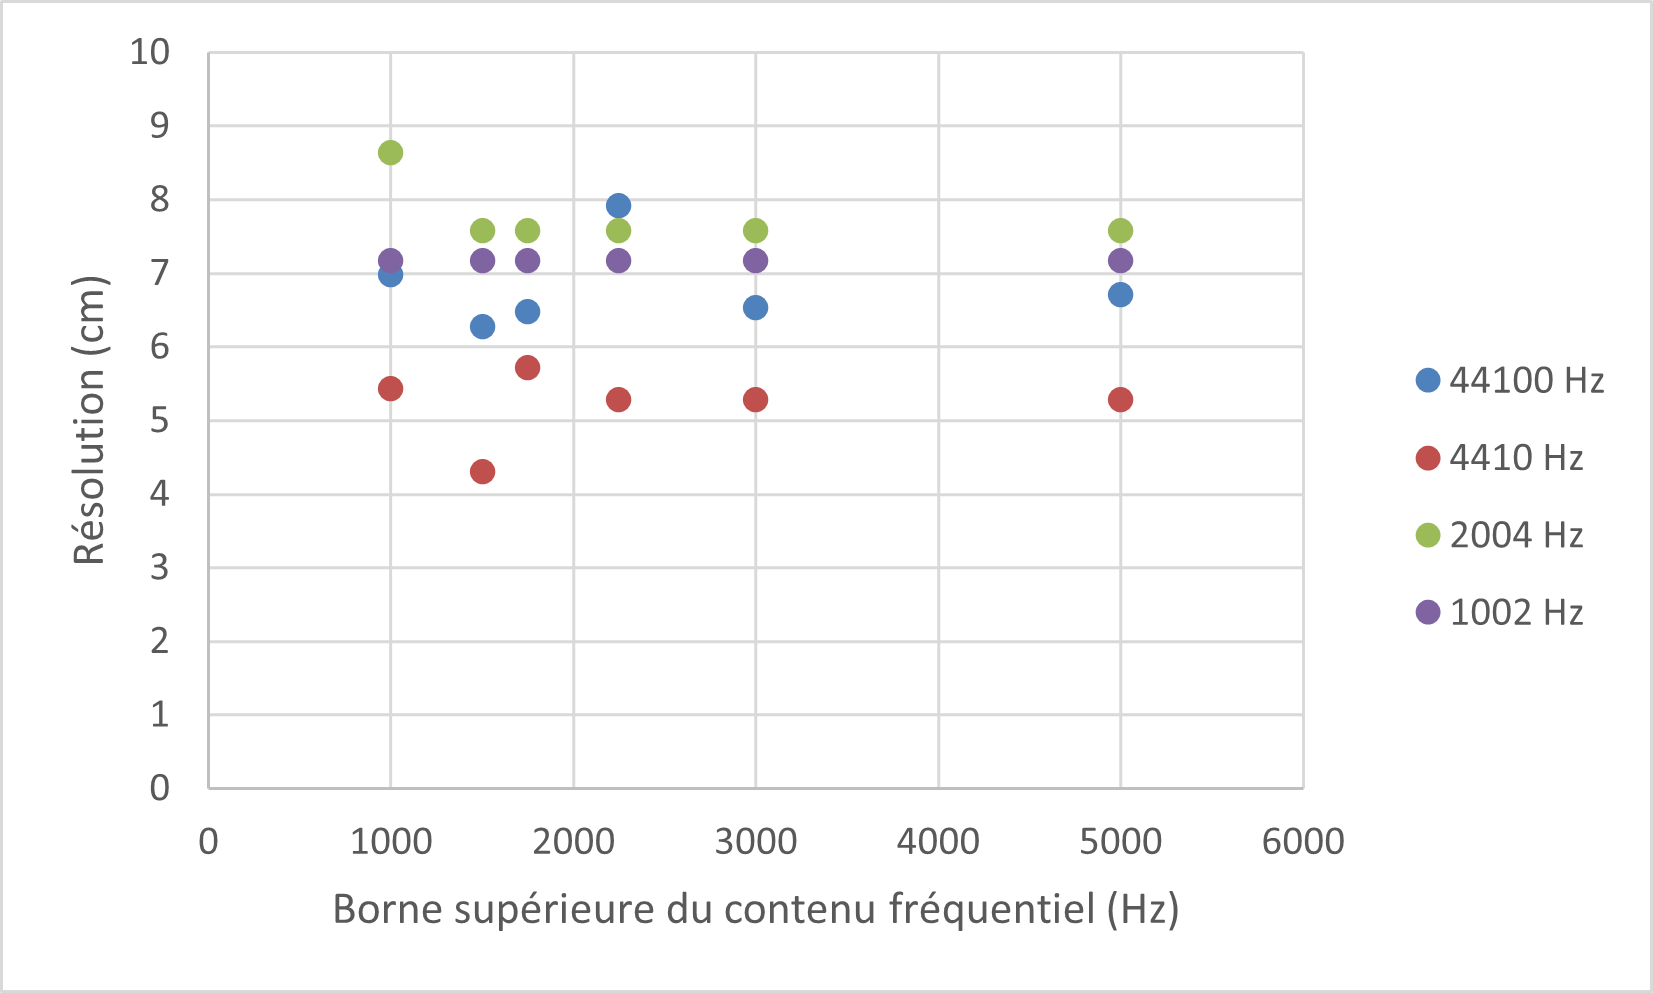
\includegraphics[scale=0.8]{resolution_interdependance.png}
    \caption{Résolution en fonction de la fréquence d'échantillonnage
    (1002, 2004, 4410 et 44100 Hz) et de la fréquence de la borne supérieure du contenu fréquentiel.
    Ici, la borne inférieure est maintenue à 300 Hz.}
    \label{res_interdep}
\end{figure}
\begin{figure}[H]
    \centering
    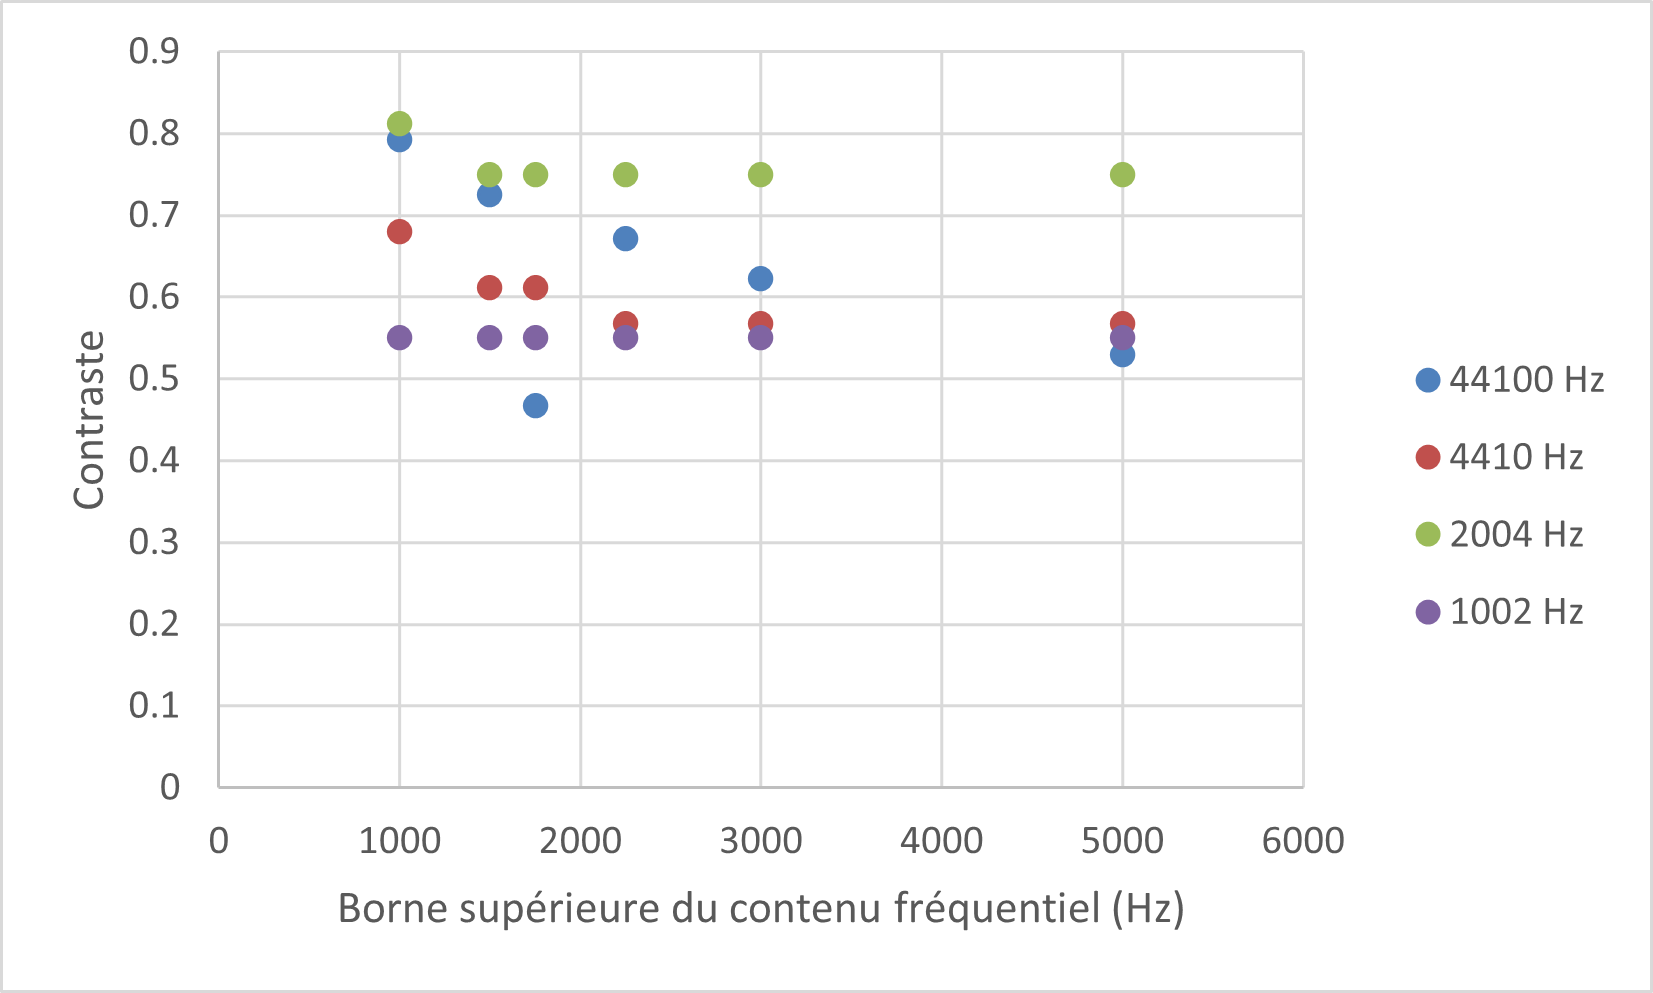
\includegraphics[scale=0.8]{contraste_interdependance.png}
    \caption{Contraste en fonction de la fréquence d'échantillonnage
    (1002, 2004, 4410 et 44100 Hz) et de la fréquence de la borne supérieure du contenu fréquentiel.
    Ici, la borne inférieure est maintenue à 300 Hz.}
    \label{contraste_interdep}
\end{figure}

En observant les tendances, on voit clairement que pour les fréquences d'échantillonnage inférieures au double
de la fréquence maximale ($f<f_{nyquist}$), les variations des valeurs de résolution et de contraste disparaissent. Par exemple,
les résultats obtenus pour une fréquence d'échantillonnage de 1002 Hz sont constants pour toutes les bornes (résolution $=7.17\ \pm \ 0.09\ cm$,
contraste $=0.551\ \pm\ 0.009$). En augmentant la fréquence d'échantillonnage, le même phénomène est observé; pour une fréquence d'échantillonnage de 
2004 Hz, tous les résultats au-dessus de $f/2=$ 1002 Hz deviennent constants et pour une fréquence d'échantillonnage de 4410 Hz, tous les résultats au-dessus de
$f/2=$ 2205 Hz deviennent constants. En dessous de la fréquence d'échantillonnage de Nyquist, les "vraies" fréquences ne sont pas détectées, mais des versions "repliée"
(\textit{aliasing}) d'elles-mêmes, à plus basse fréquence, peuvent l'être. Le phénomène est illustré dans la figure \ref{aliasing}. 
\begin{figure}[H]
    \centering
    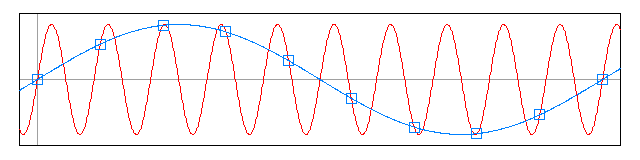
\includegraphics[scale=0.5]{Aliasing-plot.png}
    \caption{Exemple du phénomène d'\textit{aliasing} \cite{nyquist}}
    \label{aliasing}
\end{figure}

Par conséquent, il est logique que les fréquences plus grandes que $f_{sample}/2$ ne soient pas détectées, et que 
de les éliminer  à l'aide d'un filtre n'affecte d'aucune manière le résultat final. Ces tests supportent donc le fait que la fréquence 
d'acquisition de données ne doit jamais être inférieure à la fréquence de Nyquist. Si la composante fréquentielle maximale est 
connue, la fréquence d'acquisition peut dont être posée au double de celle-ci. 

\subsection{Incertitudes}\label{inc}
L'incertitude associée à l'amplitude du signal, ou l'axe-y, est celle qui provient de la résolution 
de l'ADC. La résolution de l'ADC, $\delta$, dépend du nombre de bits des échantillons, et peut être décrite par:
\[\delta=\frac{\Delta_{max}}{2^{n}},\]
où $\Delta_{max}$ est l'éventail possible des mesures, et $n$ est le nombre de bits. L'incertitude correspond
à la moitié de cette valeur, soit $\sigma_{res}=\delta/2$. L'incertitude sur la position de la source du signal
est approximée par la moitié de la largeur d'un doigt, $\sigma_{pos}\approx4\ mm$. La corrélation des signaux a été déterminée
en calculant le produit scalaire. On sait que pour une multiplication, la propagation de l'incertitude se calcule de la
manière suivante:
\begin{align*}
  \sigma_{z}=z \sqrt{\frac{\sigma_x}{x}^2+\frac{\sigma_y}{y}^2}.
\end{align*}
L'incertitude totale sur le produit scalaire est donc:
\begin{align*}
  \sigma_{tot}=\sqrt{\sum_i^{N} \sigma_{z_i}^2},
\end{align*}
où $N$ est le nombre de points évalués pour les échantillons. Pour déterminer l'incertitude sur les
paramètres du fit gaussien, tout en considérant l'impact des incertitudes en $x$ et $y$, la fonction \textit{scipy.ODR}
a été utilisée. Finalement, l'incertitude sur le contraste correspond directement à l'incertitude sur le paramètre de
l'amplitude ($\sigma_{A}$), et l'incertitude sur la résolution (FWHM) correspond à:
\begin{align*}
  \sigma_{FWHM}=\sqrt{2ln2}\ \sigma_{\sigma},
\end{align*}
où $\sigma_{\sigma}$ est l'incertitude sur l'écart-type, $\sigma$.



\section{Codes}

Les codes présentés ci-dessous ont été utilisés pour faire fonctionner le piano et pour faire les
multiples tests. Ces derniers peuvent nécessiter d'être adaptés pour pouvoir faire des tests
spécifiques, ou encore pour décider quelles notes peuvent être jouées par le piano.

\subsection{Programme pour modifier le contenu fréquentiel et la fréquence d'échantillonnage}

\begin{lstlisting}[language=python]
import numpy as np
import matplotlib.pyplot as plt
import json
import os
from scipy.optimize import curve_fit

# Charger le fichier JSON (dictionnaire de notes)
with open('C:/Users/maxim/OneDrive/Documents/GitHub/piano_project/Wav-Notes/notes_dict_1ligne.json', 'r') as f:
    data = json.load(f)
input_filepath = 'Wav-Notes/notes_dict_1ligne.json'
# Obtenir le repertoire du fichier original
output_directory = os.path.dirname(input_filepath)

# Parametres a ajuster
# liste filtre_bas : [100,100,150,150,200,200,250,250,300,300,350,350,400,400,500,500]
# liste filtre_haut : [2000,1500,2000,1500,2000,1500,2000,1500,2000,1500,2000,1500,2000,1500,2000,1500]
filtre_bas=[550]
filtre_haut=[1500]
redu=30 #facteur de reduction de la frequence d'echantillonnage

# Parametres importants
fs = int(44100//redu)  # sample rate
dt = 0.1  # Intervalle de temps (en secondes)
nb_recordings = 1  # nb d'enregistrements par note
nb_points = int(dt * fs)  # Equivalent en nombre de points pour les indices
point_du_tap = 11 # Sert a l'affichage

notes= ['1','2','3','4','5','6','7','8','9','10','11','12','13','14','15','16','17']
notes_matrix = np.zeros((len(notes) * nb_recordings, nb_points))

# Transferer les donnees du dictionnaire dans une matrice avec 17 lignes et nb_points par ligne
i = 0
for note, recordings in data.items():
    for prise in recordings:
        array = np.array(prise)
        array_fin=array[::redu]
        if len(array_fin)!=nb_points:
            array_fin=array_fin[:nb_points]
        notes_matrix[i] = array_fin
        i += 1

def dico_filtre_passband(matrice, frequence_minimale, frequence_maximale):
    # 1. Effectuer la transformee de Fourier rapide (FFT)
    signal_fft = np.fft.rfft(matrice)
    frequencies = np.fft.rfftfreq(len(matrice[0]), 1/fs)

    # 2. Creer un filtre passe-bande
    low_cutoff = frequence_minimale  # Frequence de coupure basse (Hz)
    high_cutoff = frequence_maximale  # Frequence de coupure haute (Hz)
    filter_mask = (frequencies > low_cutoff) & (frequencies < high_cutoff)

    # 3. Appliquer le filtre
    filtered_fft = signal_fft * filter_mask

    # 4. Revenir au domaine temporel avec la transformee inverse de Fourier
    filtered_signal = np.fft.irfft(filtered_fft)
    
    # 5. Remplacer la deuxieme moitie de chaque vecteur par des zeros
    filtered_signal_cut = np.zeros_like(filtered_signal)  # Creer une matrice du meme type, remplie de zeros
    half_point = filtered_signal.shape[1] // 2  # Obtenir le point de coupure (moitie)
    filtered_signal_cut[:, :half_point] = filtered_signal[:, :half_point]
    
    # Retourne le nouveau dico avec les signaux filtres
    return filtered_signal_cut, frequencies, filtered_fft[point_du_tap], signal_fft[point_du_tap]

# Fonction pour creer un nouveau fichier JSON pour chaque niveau de bits
def create_modified_json(fbas,fhaut,freq_sampling, output_directory):
    notes_dict = {}
    
    for bas,haut in zip(fbas,fhaut):
        matrice_traitee, frequencies, filtered_fft, signal_fft=dico_filtre_passband(notes_matrix,bas,haut)

    # On parcourt les notes et les enregistrements pour remplir le dictionnaire
    for i, note in enumerate(notes):
        recordings = []
        for j in range(nb_recordings):
            # On suppose que chaque enregistrement correspond a une ligne dans notes_matrix
            recordings.append(matrice_traitee[i * nb_recordings + j].tolist())  # Convertir en liste
        notes_dict[note] = recordings

    for bas,haut in zip(fbas,fhaut):
        # Generer le nom de fichier pour chaque duo de filtre
        output_filename = os.path.join(output_directory, f'fs={freq_sampling}-fbas={bas}-fhaut={haut}.json')

        # Sauvegarder le nouveau dictionnaire dans un fichier JSON
        with open(output_filename, 'w') as outfile:
            json.dump(notes_dict, outfile, indent=4)

# Creer un fichier JSON pour chaque niveau de bits dans le meme repertoire que le fichier original
create_modified_json(filtre_bas, filtre_haut, fs, output_directory)

#La suite du code n'est pas utile en soi mais permet de confirmer que ca donne la bonne chose
sign, frequencies, filtered_fft, signal_fft=dico_filtre_passband(notes_matrix,filtre_bas[0],filtre_haut[0])
signal_post_filtre=sign[point_du_tap]
signal=notes_matrix[point_du_tap]

# Generer le temps 
t1 = np.linspace(0, 1, len(signal), endpoint=False)  # Intervalle de temps
t2 = np.linspace(0, 1, len(signal_post_filtre), endpoint=False)  # Intervalle de temps
#f1, f2 = 50, 200  # Frequences des sinusoides
#signal = np.sin(2 * np.pi * f1 * t) + 0.5 * np.sin(2 * np.pi * f2 * t)

# Afficher les resultats
plt.figure(figsize=(10, 6))

# Affichage du signal original
plt.subplot(2, 2, 1)
plt.plot(t1, signal)
plt.title("Signal original")
plt.xlabel("Temps [s]")
plt.ylabel("Amplitude")

# Spectre de frequence original
plt.subplot(2, 2, 2)
plt.plot(frequencies[:fs//2], np.abs(signal_fft)[:fs//2])
plt.title("Spectre de frequence original")
plt.xlabel("Frequence [Hz]")
plt.ylabel("Amplitude")

# Spectre de frequence filtre
plt.subplot(2, 2, 4)
plt.plot(frequencies[:fs//2], np.abs(filtered_fft)[:fs//2])
plt.title("Spectre de frequence filtre")
plt.xlabel("Frequence [Hz]")
plt.ylabel("Amplitude")

# Signal filtre
plt.subplot(2, 2, 3)
plt.plot(t2, signal_post_filtre.real)
plt.title("Signal filtre")
plt.xlabel("Temps [s]")
plt.ylabel("Amplitude")

plt.tight_layout()
plt.show()
\end{lstlisting}

\subsection{Programme pour changer le nombre de bits des échantillons}

\begin{lstlisting}[language=python]
import json
import os
import numpy as np

# Charger le fichier JSON (dictionnaire)
input_filepath = 'Wav-Notes/notes_dict_1ligne.json'
with open(input_filepath, 'r') as f:
    data = json.load(f)

# Obtenir le repertoire du fichier original
output_directory = os.path.dirname(input_filepath)

# Fonction pour reduire la precision d'un signal en fonction du nombre de bits
def reduce_precision(signal, n_bits):
    if n_bits == 1:
        # Cas special pour 1 bit : toutes les valeurs negatives deviennent 0
        return [1 if value > 0 else 0 for value in signal]
    elif n_bits > 1:
        levels = 2**(n_bits - 1)  # Utiliser n_bits - 1 pour tenir compte du bit de signe
        # Quantifier le signal dans le nombre de niveaux approprie
        signal_quantified = np.round(np.array(signal) * (levels // 2)) / (levels // 2)
    else:
        signal_quantified = np.zeros_like(signal)  # Tout est ramene a zero pour 0 bit
    
    return signal_quantified.tolist()  # Convertir en liste pour garder le format JSON

# Fonction pour creer un nouveau fichier JSON pour chaque niveau de bits
def create_modified_json(data, n_bits, output_directory):
    # Creer un nouveau dictionnaire avec les signaux modifies
    modified_data = {}
    
    for note, vecteurs in data.items():
        modified_data[note] = [reduce_precision(vecteur, n_bits) for vecteur in vecteurs]
    
    # Generer le nom de fichier pour chaque niveau de bits
    output_filename = os.path.join(output_directory, f'modified_signal_{n_bits}bit.json')
    
    # Sauvegarder le nouveau dictionnaire dans un fichier JSON
    with open(output_filename, 'w') as outfile:
        json.dump(modified_data, outfile, indent=4)

# Creer un fichier JSON pour chaque niveau de bits dans le meme repertoire que le fichier original
create_modified_json(data, 16, output_directory)
create_modified_json(data, 8, output_directory)
create_modified_json(data, 6, output_directory)
create_modified_json(data, 4, output_directory)
create_modified_json(data, 3, output_directory)
create_modified_json(data, 2, output_directory)
create_modified_json(data, 1, output_directory)
create_modified_json(data, 0, output_directory)
\end{lstlisting}

\subsection{Programme pour calculer la résolution et le contraste pour un dictionnaire de notes}

\begin{lstlisting}[language=python]
import numpy as np
from scipy.odr import ODR, Model, RealData
import json
import pandas as pd
from scipy.optimize import curve_fit
import matplotlib.pyplot as plt
print('Librairies importees')

# liste des noms de dictionnaires JSON a charger
fichiers=['notes_dict_1ligne','modified_signal_1bit','modified_signal_2bit','modified_signal_3bit'
          ,'modified_signal_4bit','modified_signal_6bit','modified_signal_8bit','modified_signal_16bit']

# Charger les fichiers JSON
def lecteur():
    encyclopedie=[]
    for nom in fichiers:
        with open(f'Wav-Notes/{nom}.json', 'r') as f:
            encyclopedie.append(json.load(f))
    return encyclopedie 

# Fonction gaussienne avec floor ajustable pour curve_fit
def gaussian_with_floor(x, A, mu, sigma, floor):
    return A * np.exp(-((x - mu) ** 2) / (2 * sigma ** 2)) + floor

# Fonction pour ajuster avec des bornes (curve_fit)
def fit_gaussian_with_bounds(corr_data, xaxis, yerr):
    x_data = xaxis  # np.arange(len(corr_data))
    initial_guess = [np.max(corr_data), np.argmax(corr_data), np.std(corr_data), np.mean(corr_data)]  # [amplitude, mean, sigma, offset]

    # Contraintes sur les bornes pour que sigma > 0 et floor proche de la moyenne des donnees
    bounds = ([0, 0, 0, np.mean(corr_data) - 0.09], [np.inf, len(corr_data), np.inf, np.mean(corr_data) + 0.09])

    # Utilisation de curve_fit avec la nouvelle fonction gaussienne
    params, pcov = curve_fit(gaussian_with_floor, x_data, corr_data, p0=initial_guess,
                             sigma=yerr, absolute_sigma=True, bounds=bounds, maxfev=10000)

    perr = np.sqrt(np.diag(pcov))  # Erreurs sur les parametres ajustes
    return params, perr, x_data

# Fonction pour calculer la correlation du curve_fit
def correlateur_et_curve_fit_gaussien(data, point_du_tap):
        #Rembarque sur le code a Marielou
    # Parametres importants
    nb_points = len(data['1'][0])  
    dt = 0.1
    fs=int(nb_points/dt) # sample rate
    nb_recordings = 1  # nb d'enregistrements par note

    notes = ['1','2','3','4','5','6','7','8','9','10','11','12','13','14','15','16','17']
    matrice = np.zeros((len(notes) * nb_recordings, nb_points))

    i = 0
    for note, recordings in data.items():
        for prise in recordings:
            array = np.array(prise)
            array_normalise = array / np.max(array)
            matrice[i] = array_normalise
            i += 1

    signaux_reference = matrice
    signal = matrice[point_du_tap]
    position = 3*10**(-2) + 1.5*np.arange(0, 17)*10**(-2)
    correlation = np.dot(signaux_reference,signal)/np.max(np.dot(signaux_reference,signal))

    nb_bits = 32
    range = 2
    err_ampl = (range/(2**(nb_bits)))/2

    # Propagation de l'erreur sur le produit scalaire de la correlation
    yerr = []
    for element in signaux_reference:
        # Remplacer les zeros par une petite valeur pour eviter la division par zero
        signal_safe = np.where(signal == 0, 1e-10, signal)
        element_safe = np.where(element == 0, 1e-10, element)

        # Calculer l'erreur de multiplication
        err_multiplication = (signal_safe * element_safe) * np.sqrt((err_ampl / signal_safe) ** 2 + (err_ampl / element_safe) ** 2)

        # Verifier si err_multiplication contient des NaN ou des infinis
        if np.any(np.isnan(err_multiplication)) or np.any(np.isinf(err_multiplication)):
            print("Attention : err_multiplication contient des NaN ou des infinis.")
            continue  # Passer a l'iteration suivante

        # Calculer l'erreur totale
        err_prod = np.sqrt(np.sum(err_multiplication ** 2))
        yerr.append(err_prod)
    #yerr=1*correlation

    params, perr, x_data = fit_gaussian_with_bounds(correlation,position, yerr)
    
    amplitude_fit, mean_fit, sigma_fit, offset_fit = params
    amplitude_err, mean_err, sigma_err, offset_err = perr

    # La resolution est convertie en cm (chaque point est espace de 1,5 cm)
    resolution = 1.5 * np.log(2) * np.sqrt(2) * sigma_fit
    resolution_err = 1.5 * np.log(2) * np.sqrt(2) * sigma_err

    max_diff = amplitude_fit-offset_fit
    max_diff_err = amplitude_err-offset_err

    return {
        "resolution": resolution,
        "resolution_err": resolution_err,
        "max_diff": max_diff,
        "max_diff_err": max_diff_err,
    }

# Fonction gaussienne ODR
def gaussian_with_floor_constrained(p, x):
    A, mu, log_sigma, floor = p
    sigma = np.exp(log_sigma)  # sigma > 0 en utilisant la transformation exponentielle
    return A * np.exp(-((x - mu) ** 2) / (2 * sigma ** 2)) + floor

# Fonction pour calculer la correlation ODR
def correlateur_ODR(data,point_du_tap,nb_bit):
    # Parametres importants
    nb_points = len(data['1'][0])  
    dt = 0.1
    fs=int(nb_points/dt) # sample rate
    nb_recordings = 1  # nb d'enregistrements par note

    notes = ['1','2','3','4','5','6','7','8','9','10','11','12','13','14','15','16','17']
    matrice = np.zeros((len(notes) * nb_recordings, nb_points))

    i = 0
    for note, recordings in data.items():
        for prise in recordings:
            array = np.array(prise)
            array_normalise = array / np.max(array)
            matrice[i] = array_normalise
            i += 1

    signaux_reference = matrice
    signal = matrice[point_du_tap]
    position = 3*10**(-2) + 1.5*np.arange(0, 17)*10**(-2)
    correlation = np.dot(signaux_reference,signal)/np.max(np.dot(signaux_reference,signal))

    nb_bits = nb_bit
    range = 2
    err_ampl = (range/(2**(nb_bits)))/2
    err_position = 4e-3

    # Propagation de l'erreur sur le produit scalaire de la correlation
    err_prod_ampl = []
    for element in signaux_reference:
        # Remplacer les zeros par une petite valeur pour eviter la division par zero
        signal_safe = np.where(signal == 0, 1e-10, signal)
        element_safe = np.where(element == 0, 1e-10, element)

        # Calculer l'erreur de multiplication
        err_multiplication = (signal_safe * element_safe) * np.sqrt((err_ampl / signal_safe) ** 2 + (err_ampl / element_safe) ** 2)

        # Verifier si err_multiplication contient des NaN ou des infinis
        if np.any(np.isnan(err_multiplication)) or np.any(np.isinf(err_multiplication)):
            print("Attention : err_multiplication contient des NaN ou des infinis.")
            continue  # Passer a l'iteration suivante

        # Calculer l'erreur totale
        err_prod = np.sqrt(np.sum(err_multiplication ** 2))
        err_prod_ampl.append(err_prod)

    # Utilisation de ODR pour faire le fit gaussien avec sigma toujours positif
    data = RealData(position, correlation, sx=err_position, sy=err_prod_ampl)
    model = Model(gaussian_with_floor_constrained)
    
    guess_initial = [np.max(correlation), np.mean(position), np.log(np.std(position)), np.mean(correlation)]
    odr = ODR(data, model, beta0=guess_initial)
    output = odr.run()

    # Parametres optimaux et matrice de covariance
    A_opt, mu_opt, log_sigma_opt, floor_opt = output.beta
    sigma_opt = np.exp(log_sigma_opt)  # Revenir a sigma

    resolution = np.sqrt(2 * np.log(2)) * sigma_opt
    resolution_err = np.sqrt(2 * np.log(2)) * sigma_opt * np.sqrt(output.cov_beta[2, 2])

    contraste = A_opt-np.mean(correlation)
    contraste_err = 2*np.sqrt(output.cov_beta[0, 0])
    
    return {
        "resolution": resolution,
        "resolution_err": resolution_err,
        "max_diff": contraste,
        "max_diff_err": contraste_err,
    }

    # Ajuster les donnees avec la fonction gaussienne avec plancher
    params, perr, x_data = fit_gaussian_with_offset_and_errors(corr_data, yerr)
    
    # Extraction des parametres ajustes
    amplitude_fit, mean_fit, sigma_fit, offset_fit = params
    amplitude_err, mean_err, sigma_err, offset_err = perr

    # La resolution est convertie en cm (chaque point est espace de 1,5cm)
    resolution = 1.5 * np.log(2) * np.sqrt(2) * sigma_fit
    resolution_err = 1.5 * np.log(2) * np.sqrt(2) * sigma_err  

    # Calcul de la difference entre le maximum de la gaussienne et l'offset
    max_diff = amplitude_fit
    max_diff_err = amplitude_err  # Incertitude sur la difference est celle de l'amplitude

    # Retourner les resultats
    return {
        "resolution": resolution,
        "resolution_err": resolution_err,
        "max_diff": max_diff,
        "max_diff_err": max_diff_err,
    }

# Creer une liste pour stocker les resultats
results_list = []
dictionaries_to_process = lecteur()  # Ajoute les autres dictionnaires ici
bit_names = ['Original', '1bit', '2bit', '3bit', '4bit', '6bit', '8bit', '16bit']
bit_qty = [32, 1, 2, 3, 4, 6, 8, 16]  # bit_qty[idx]

for idx, current_data in enumerate(dictionaries_to_process):
    a1 = []
    a2 = []
    a3 = []
    a4 = []
    for i in [7, 8, 9, 10, 11]:
        corr_data = correlateur_ODR(current_data, i, bit_qty[idx])

        # Analyser les ajustements
        results = corr_data
        a1.append(results["resolution"])
        a2.append(results["resolution_err"])
        a3.append(results["max_diff"])
        a4.append(results["max_diff_err"])

    resolution = np.mean(a1)
    resolution_err = np.mean(a2)
    contraste = np.mean(a3)
    contraste_err = np.mean(a4)

    # Ajouter les resultats a la liste, en incluant les noms des bits
    results_list.append({
        "Dictionnaire": bit_names[idx],
        "Resolution": resolution,
        "Erreur Resolution": resolution_err,
        "Contraste": contraste,
        "Erreur Contraste": contraste_err,
    })

# Convertir les resultats en DataFrame
results_df = pd.DataFrame(results_list)

# Exporter les resultats en fichier Excel
results_df.to_excel('resultats_nouveaux_points_nb_bit.xlsx', index=False)

print("Analyse terminee et resultats exportes vers 'resultats'.")
\end{lstlisting}

\subsection{Programme pour enregistrer un dictionnaire de notes}

\begin{lstlisting}[language=python]
import sounddevice as sd
import numpy as np
import json

# temps pour taper la note
seconds = 2 

# freq d'acquisition par defaut
fs = 44100    

default = True # Si cette option est utilisee, le micro/speaker par defaut est utilise
devices = sd.query_devices()

if not default:
    InputStr = "Choisir le # correspondant au micro parmi la liste: \n"
    OutputStr = "Choisir le # correspondant au speaker parmi la liste: \n"
    for i in range(len(devices)):
        if devices[i]['max_input_channels']:
            InputStr += ('%d : %s \n' % (i, ''.join(devices[i]['name'])))
        if devices[i]['max_output_channels']:
            OutputStr += ('%d : %s \n' % (i, ''.join(devices[i]['name'])))
    DeviceIn = input(InputStr)
    DeviceOut = input(OutputStr)

    sd.default.device = [int(DeviceIn), int(DeviceOut)]

# liste de notes a enregistrer
notes = ['1','2','3','4','5','6','7','8','9','10','11','12','13','14','15','16','17']

notes_dict = {note: None for note in notes}
dt = 1e-1  # Intervalle de temps (en secondes)
nb_points = int(dt*fs) # Equivalent en nombre de points pour les indices

# enregistrement de chaque note
for note in notes:
    recordings = []
    print(f'Enregistrement de la note', note)

    # ecoute de la note
    myrecording = sd.rec(int(seconds * fs), samplerate=fs, channels=1)
    sd.wait()
    print(f'Enregistrement fini.')

    # Trouver l'amplitude maximale en valeur absolue
    max_amplitude = np.max(abs(myrecording))
    threshold = max_amplitude / 10  # Definir le seuil
    print(threshold)

    # Creer la fenetre utilisee pour le signal
    for index, value in enumerate(myrecording):
        if value >= threshold:
            start_signal = index
            break

    cut_signal = myrecording[start_signal:(start_signal + nb_points)].flatten()

    # Normalisation du signal
    norm_cut_signal = cut_signal / max_amplitude

    # Rajouter le nouveau array a la liste 'recordings'
    recordings.append(norm_cut_signal.tolist())

    # Transformer la liste en array
    nom_note = note
    notes_dict[nom_note] = recordings

# sauvegarde du dictionnaire en JSON
with open('notes_dict_1ligne.json', 'w') as json_file:
    json.dump(notes_dict, json_file)
\end{lstlisting}

\subsection{Programme pour jouer du piano en temps réel}

\begin{lstlisting}[language=python]
import sounddevice as sd
import numpy as np
import threading
import matplotlib.pyplot as plt
import time
from collections import deque
import pygame
from pydub import AudioSegment
import os
import json
import math

# chargement du dictionnaire
with open('Wav-Notes\\notes_dict_jo.json', 'r') as file:
    data = json.load(file)

# parametres audio
fs = 44100 
dt = 0.1  # Intervalle de temps (en secondes)
nb_recordings = 1 # Combien de signaux par note
nb_points = int(dt * fs)

# liste de notes
notes = ['1', '2', '3', '4', '5', '6', '7', '8', '9', '10', '11', '12', '13', '14', '15', '16', '17']
notes_matrix = np.zeros((len(notes) * nb_recordings, nb_points))

# Conversion des donnees en arrays et reformatage de la memoire
i = 0
for note, recordings in data.items():
    for element in recordings:
        array = np.array(element) 
        notes_matrix[i] = array
        i += 1

notes_dict = {
    '1': 'c3.wav',
    '2': 'c-3.wav',
    '3': 'd3.wav',
    '4': 'd-3.wav',
    '5': 'e3.wav',
    '6': 'f3.wav',
    '7': 'f-3.wav',
    '8': 'g3.wav',
    '9': 'g-3.wav',
    '10': 'a4.wav',
    '11': 'a-4.wav',
    '12': 'b4.wav',
    '13': 'c4.wav',
    '14': 'c-4.wav',
    '15': 'd4.wav',
    '16': 'd-4.wav',
    '17': 'e4.wav'
}

pygame.mixer.init()

# THREAD : fonction pour jouer l'audio d'une note
def jouer_note(note):
    if note in notes_dict:
        fichier_note = f'Wav-Notes\\{notes_dict[note]}'
        
        if os.path.isfile(fichier_note):
            # Load the WAV file in memory
            note_sound = AudioSegment.from_wav(fichier_note)
            
            # Play the note using pygame
            son = pygame.mixer.Sound(fichier_note)
            son.play()
            pygame.time.wait(int(note_sound.duration_seconds * 1000))  # attendre fin de l'audio
        else:
            print(f"Le fichier {fichier_note} n'existe pas.")
    else:
        print("Note non reconnue.")

# test de note
jouer_note('c3')

# parametres de detection de signal audio
threshold = 0.01  # amplitude minimale pour signaler une impulsion
spike_detected = False  # flag pour savoir si un signal est detecte
capture_duration = 0.15  # temps de capture d'audio post impulsion
buffer_size = fs  # taille du buffer qui contient le signal audio roulant
signal_buffer = np.zeros(buffer_size)

# Au besoin, fonction pour visualiser le signal audio d'une impulsion
def plot_data(data):
    t = np.linspace(0, dt, len(data))
    plt.plot(t, data)
    plt.xlabel('Time [s]')
    plt.ylabel('Amplitude')
    plt.title('Signal After Spike')
    plt.show()

# Lecture d'audio en temps reel
def audio_callback(indata, frames, time, status):
    global spike_detected, signal_buffer
    
    if status:
        print(status)
    
    # aplatissage du data entrant
    audio_data = indata[:, 0]
    
    # roulement du signal dans le buffer
    signal_buffer = np.roll(signal_buffer, -frames)
    signal_buffer[-frames:] = audio_data
    
    # Analyse du buffer pour l'impulsion
    if not spike_detected and np.max(audio_data) > threshold:
        spike_detected = True
        print("Spike detected!")
    
        # Si detection, lance le thread d'analyse de signal
        capture_thread = threading.Thread(target=signal_analysis)
        capture_thread.start()

# THREAD : Analyse de signal
def signal_analysis():
    global spike_detected
    
    time.sleep(capture_duration)  # laisse le buffer prendre la suite du signal post impulsion

    # Capture du signal de l'impulsion dans le buffer
    post_spike_data = np.copy(signal_buffer)[int(fs - fs * capture_duration - 800):]
    
##################################################################
# Traitement de donnees
##################################################################

    data_max_amp = np.max(abs(post_spike_data))
    data_threshold = data_max_amp / 10

    # Creer la fenetre utilisee pour le signal
    for index, value in enumerate(post_spike_data):
        if value >= data_threshold:
            start_signal = index
            break
    cut_data = post_spike_data[start_signal:(start_signal + int(dt * fs))].flatten()

    # Plot the data
    # plot_data(cut_data)

    # Normalisation du signal
    norm_cut_data = cut_data / data_max_amp

    # Transformer la liste en array
    signal_array = np.array(norm_cut_data)

    # Produit scalaire (correlation) entre les donnees de training et le signal test
    scalar_prod = np.dot(notes_matrix, signal_array)

    # Trouver l'indice de la valeur max du produit scalaire et trouver sa note correspondante
    index_max = np.argmax(scalar_prod)
    note_index = index_max // nb_recordings
    print(scalar_prod)

    note = notes[note_index]
    if note:
        print(f"Playing note: {note}")
        # Lance le thread pour jouer la note identifiee
        play_note_thread = threading.Thread(target=jouer_note, args=(note,))
        play_note_thread.start()
    
    # Reset du flag pour continuer a lire des impulsions
    spike_detected = False

# Lancement de la lecture d'audio en continu
with sd.InputStream(callback=audio_callback, samplerate=fs, channels=1):
    print("Recording... (Press Ctrl+C to stop)")
    while True:
        time.sleep(0.001)  # Keep the main loop running
\end{lstlisting}

\clearpage
\section{Annexe}

\subsection{Preuve de la correction par Antidote}

Cette capture d'écran prouve que le contenu de cette fiche technique a été vérifié par
le logiciel Antidote pour la correction du français.


\clearpage
\printbibliography
% \bibliographystyle{unsrtnat}
% \bibliography{My_Library}

\end{document}
